
In diesem Kapitel sind die Sequenzdiagramme beschrieben, die Vorgänge beschreiben, deren Verhalten nicht trivial ist.
Nicht trivial ist ein Verhalten, bei dem der Ablauf des Diagramms nicht einem ``Durchreichen'' von Aufrufen entspricht.
\section{Triviale Abfrage}
\begin{figure}[H]
	\centering
	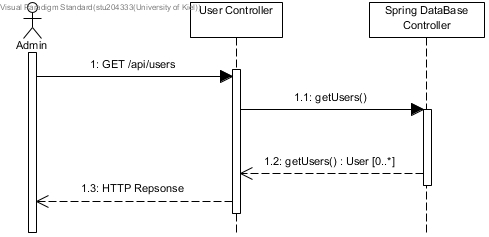
\includegraphics[width = 12cm]{img/diagrams/TrivialDiagram}
	\caption{Abfrage der Nutzerlisten}
\end{figure}
Als Beispiel für ein triviales Sequenzdiagramm lässt sich das Abfragen der Daten durch einen Admin hernehmen. Dabei beschreibt ``User [0..*]'' die Rückgabe eines ``UserList DTO''.
 
\section{Bilder in der App übermitteln}
\begin{figure}[H]
	\centering
	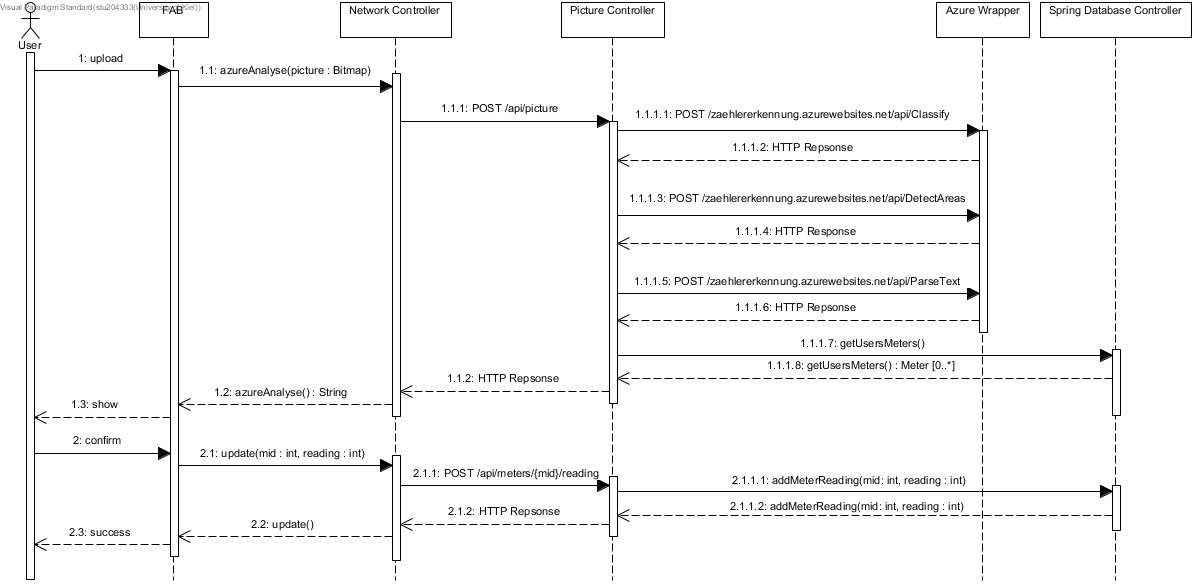
\includegraphics[width=16cm]{img/diagrams/SubmitFotoSequence}
	\caption{Erfolgreiche Bildübermittlung}
\end{figure}
Das folgende Sequenzdiagramm beschreibt den Vorgang des erfolgreichen Übermittelns eines Zählerstandes als Bild.
Zuerst lädt der Nutzer ein Foto hoch, dieses wird mittels der Methode azureAnalyse() vom Netzwerk-Controller per POST-Request ans Back-End der Website geschickt. Dieses leitet das Bild per HTTP an die Klassifizierungsschnittstelle des AzureWrappers weiter. Nach der Antwort wird über HTTP das Bild an die nächste Schnittstelle, ``Area Detect'' geschickt. Als Letztes wird das Bild via HTTP an die Schnittstelle ``Parse Text''  geschickt. Die erhaltenen Daten werden jetzt einer ersten Plausibilitätsprüfung unterzogen. Die wird die Richtigkeit der Länge und der Klassifizierung überprüft.\\
Nun werden mittels getUsersMeters() alle Zähler für den Nutzer abgefragt, um zu Prüfen, ob die Nummer des Zählers der Nummer eines der Zähler des Users entspricht.
Wenn dies der Fall ist, wird eine HTTP-Response an den Network-Controller gesendet, die die gelesene Zählernummer und den gelesenen Zählerstand übermittelt. Nun wird der Nutzer aufgefordert die gelesenen Werte zu bestätigen. \\
Der Ablauf eines manuellen Eintrages entspricht dem unteren Teil des Diagramms (ab Punkt 2).

\section{Zählerstände für User updaten}
\begin{figure}[H]
	\centering
	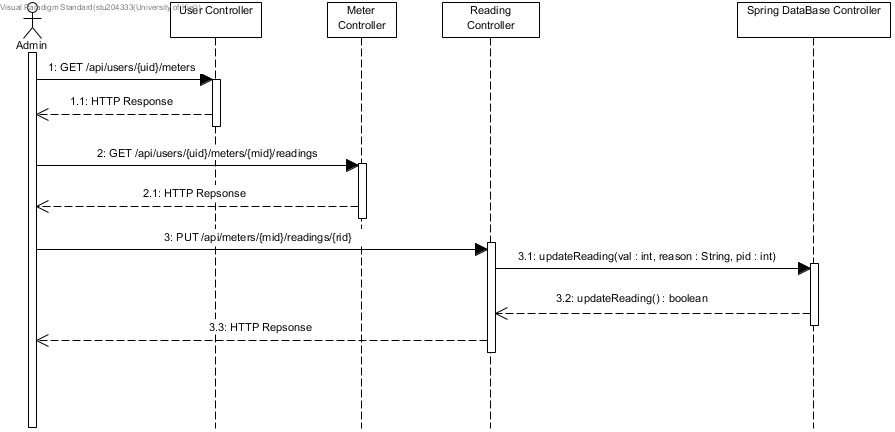
\includegraphics[width = 15cm]{img/diagrams/ChangeReading}
	\caption{Zählerstand eines Nutzers als Admin updaten}
\end{figure}
Administratoren können unter Angabe eines Grundes Zählerstände aktualisieren.
Dafür muss der Administrator zuerst mittels eines HTTP-Requests alle Zähler  zu einer User-ID vom UserController abfragen. Danach werden mittels einer weiteren Anfrage alle Zählerstände des Zählers abgefragt. Nun kann mittels eines PUT-Request mit der Reading-ID ein bestimmter Eintrag verändert werden. Dafür wird der neue Zählerstand, der Grund der Änderung und die ID des Admins versendet, die dann für den Funktionsaufruf ''updateReading'' verwendet wird. Wenn die Änderung erfolgreich war, sendet der Reading Controller in der HTTP Response einen Erfolg zurück.